\documentclass[aspectratio=169, 10pt]{beamer}

% ==============================================================================
% Preamble Configuration for Risk-Aware RL Beamer Presentation (INT3011E)
% ==============================================================================

\usepackage[utf8]{inputenc}
\usepackage[vietnamese]{babel}
\usepackage{amsmath, amssymb, amsfonts}
\usepackage{booktabs}
\usepackage{multicol}
\usepackage{multirow}
\usepackage{graphicx}
\usepackage{xcolor}
\usepackage{colortbl}
\usepackage{hyperref}
\usepackage{tikz}
\usetikzlibrary{shapes.geometric, arrows.meta, positioning, calc, fit, backgrounds}

% --- Custom Corporate & Academic Quant Color Palette ---
\definecolor{MainNavy}{RGB}{14, 34, 61}        % Primary Header & Strong emphasis
\definecolor{SecondaryNavy}{RGB}{28, 64, 110}  % Block titles
\definecolor{AccentCyan}{RGB}{2, 132, 199}      % Highlighting and links
\definecolor{AlertCrimson}{RGB}{220, 38, 38}   % Risk / Drawdown / Pain points
\definecolor{SuccessGreen}{RGB}{22, 163, 74}    % Overperformance / Solved
\definecolor{BgSoftGray}{RGB}{248, 250, 252}    % Subtle block background
\definecolor{BorderGray}{RGB}{226, 232, 240}    % Card borders
\definecolor{DarkText}{RGB}{30, 41, 59}         % Text color

% --- Theme Customization ---
\usetheme{Madrid}
\usecolortheme{whale}

% Beamer element color adjustments
\setbeamercolor{palette primary}{bg=MainNavy, fg=white}
\setbeamercolor{palette secondary}{bg=SecondaryNavy, fg=white}
\setbeamercolor{palette tertiary}{bg=AccentCyan, fg=white}
\setbeamercolor{title}{bg=MainNavy, fg=white}
\setbeamercolor{frametitle}{bg=MainNavy, fg=white}
\setbeamercolor{structure}{fg=SecondaryNavy}
\setbeamercolor{normal text}{fg=DarkText}

% Block Colors
\setbeamercolor{block title}{bg=SecondaryNavy, fg=white}
\setbeamercolor{block body}{bg=BgSoftGray, fg=DarkText}

\setbeamercolor{block title alerted}{bg=AlertCrimson, fg=white}
\setbeamercolor{block body alerted}{bg=AlertCrimson!5, fg=DarkText}

\setbeamercolor{block title example}{bg=SuccessGreen, fg=white}
\setbeamercolor{block body example}{bg=SuccessGreen!5, fg=DarkText}

% Remove default navigation symbols
\setbeamertemplate{navigation symbols}{}

% Clean and professional footline
\setbeamertemplate{footline}{
  \leavevmode%
  \hbox{%
    \begin{beamercolorbox}[wd=.6\paperwidth,ht=2.4ex,dp=1ex,left,leftskip=1.2em]{palette primary}%
      \textbf{Báo Cáo Đề Tài:} Risk-Aware RL cho Danh Mục VN30
    \end{beamercolorbox}%
    \begin{beamercolorbox}[wd=.4\paperwidth,ht=2.4ex,dp=1ex,right,rightskip=1.2em]{palette primary}%
      Trang \insertframenumber{} / \inserttotalframenumber
    \end{beamercolorbox}%
  }%
  \vskip0pt%
}

% Itemize bullet styling
\setbeamertemplate{itemize item}{\color{AccentCyan}$\blacktriangleright$}
\setbeamertemplate{itemize subitem}{\color{SecondaryNavy}$\bullet$}
\setbeamertemplate{enumerate item}{{\color{SecondaryNavy}\textbf{\insertenumlabel.}}}

% Custom Macro Boxes
\newcommand{\alertcard}[2]{
  \begin{alertblock}{#1}
    #2
  \end{alertblock}
}

\newcommand{\successcard}[2]{
  \begin{exampleblock}{#1}
    #2
  \end{exampleblock}
}

\newcommand{\kpicard}[3]{
  \begin{block}{#1}
    \centering
    {\Large \color{AccentCyan}\textbf{#2}}\\[0.2ex]
    {\footnotesize \color{DarkText}#3}
  \end{block}
}


% --- Metadata (Chỉ giữ Tên đề tài, loại bỏ hoàn toàn tên thành viên, khoa, học phần) ---
\title[\textbf{Risk-Aware RL cho VN30}]{\huge \textbf{Học Tăng Cường Nhận Thức Rủi Ro}}
\subtitle{\Large Ứng Dụng Trong Tối Ưu Hóa Phân Bổ Danh Mục Cổ Phiếu VN30 (Sàn HOSE)}
\author{}
\institute{}
\date{\normalsize Báo Cáo Nghiên Cứu Đề Tài --- 2026}

% ==============================================================================
% PRESENTATION SLIDES
% ==============================================================================
\begin{document}

% ------------------------------------------------------------------------------
% Slide 1: Title Page (Tối giản, chỉ hiện tên đề tài, sang trọng và hiện đại)
% ------------------------------------------------------------------------------
\begin{frame}[plain]
  \vspace{3.5em}
  \begin{center}
    {\color{MainNavy}\huge \textbf{HỌC TĂNG CƯỜNG NHẬN THỨC RỦI RO}}\\[0.8ex]
    {\color{SecondaryNavy}\Large \textbf{(Risk-Aware Reinforcement Learning)}}\\[1.5ex]
    {\color{AccentCyan}\rule{0.5\textwidth}{1.5pt}}\\[2.5ex]
    {\large \textbf{Bài toán phân bổ danh mục đầu tư rổ cổ phiếu VN30 trên sàn HOSE}}\\[1.5ex]
    {\normalsize \textit{Tối ưu hóa lợi nhuận bền vững và kiểm soát sụt giảm tài sản}}\\[4ex]
    
    {\footnotesize \color{gray} Báo Cáo Tiến Độ Đề Tài $\bullet$ 2026}
  \end{center}
\end{frame}

% ------------------------------------------------------------------------------
% Slide 2: Outline (4 phần dễ nắm bắt)
% ------------------------------------------------------------------------------
\begin{frame}{Nội Dung Báo Cáo Hôm Nay}
  \begin{columns}[t]
    \begin{column}{0.48\textwidth}
      \begin{block}{\textbf{Phần 1: Thực Trạng \& Vấn Đề}}
        \begin{itemize}
          \item Tại sao đầu tư chứng khoán lại khó?
          \item "Tử huyệt" của các Bot AI thông thường
          \item Luật chơi khắt khe tại thị trường Việt Nam (HOSE)
        \end{itemize}
      \end{block}

      \vspace{0.8ex}
      \begin{block}{\textbf{Phần 2: Ý Tưởng Giải Pháp}}
        \begin{itemize}
          \item Xây dựng Bot AI "Biết Sợ Rủi Ro"
          \item Nguyên lý ra quyết định: "Chiếc bánh 100\%"
          \item Sàn đấu giả lập Gymnasium cho AI
        \end{itemize}
      \end{block}
    \end{column}

    \begin{column}{0.48\textwidth}
      \begin{block}{\textbf{Phần 3: Cách Thức Vận Hành}}
        \begin{itemize}
          \item Kiến trúc tổng thể 4 bước
          \item Hai "học trò AI": Thuật toán PPO \& SAC
          \item Các tiêu chí đánh giá thành công (KPI)
        \end{itemize}
      \end{block}

      \vspace{0.8ex}
      \begin{block}{\textbf{Phần 4: Tiến Độ \& Kế Hoạch}}
        \begin{itemize}
          \item Dữ liệu thực tế 7 năm rổ VN30
          \item Tiến độ hiện tại \& Giai đoạn tiếp theo
        \end{itemize}
      \end{block}
    \end{column}
  \end{columns}
\end{frame}

% ------------------------------------------------------------------------------
% Slide 3: Real problem in investing
% ------------------------------------------------------------------------------
\begin{frame}{1. Thực Trạng: Tại Sao Đầu Tư Chứng Khoán Lại Khó?}
  \begin{columns}[c]
    \begin{column}{0.50\textwidth}
      \alertcard{Tâm lý con người trong thị trường}{
        \begin{itemize}
          \item \textbf{Hưng phấn (FOMO):} Thấy cổ phiếu tăng trần thì đổ xô mua đu đỉnh.
          \item \textbf{Hoảng loạn \& Gồng lỗ:} Khi thị trường sập thì sợ hãi bán tháo đúng đáy hoặc ôm hy vọng "rồi nó sẽ hồi".
          \item \textbf{Kết quả:} Đa số nhà đầu tư cá nhân thua lỗ nặng nề qua các đợt khủng hoảng.
        \end{itemize}
      }
    \end{column}

    \begin{column}{0.48\textwidth}
      \begin{block}{Các cú sốc khốc liệt tại Việt Nam}
        \begin{itemize}
          \item \textbf{Năm 2022 (Đại suy thoái):}
            \begin{itemize}
              \item VN-Index rơi từ 1.528 về 873 điểm (\textbf{giảm 43\%}).
              \item HPG từ 44k $\to$ 12k; SSI từ 45k $\to$ 13k (chia 3, chia 4).
            \end{itemize}
          \vspace{0.5ex}
          \item \textbf{Tháng 03/2020 (Dịch COVID-19):}
            \begin{itemize}
              \item Giảm 33\% chỉ trong 4 tuần; trắng bên mua liên tiếp nhiều phiên.
            \end{itemize}
        \end{itemize}
      \end{block}
    \end{column}
  \end{columns}

  \vspace{1ex}
  \begin{center}
    {\color{MainNavy}\textbf{Bài học cốt tử:}} Kiếm được tiền lúc thị trường tăng rất dễ, nhưng \textbf{giữ được tiền khi thị trường sập} mới là yếu tố quyết định sống còn!
  \end{center}
\end{frame}

% ------------------------------------------------------------------------------
% Slide 4: AI Failure modes (Why traditional AI fails)
% ------------------------------------------------------------------------------
\begin{frame}{2. "Tử Huyệt" Của Các Bot AI Thông Thường}
  \begin{columns}[c]
    \begin{column}{0.50\textwidth}
      \begin{block}{Bot AI thông thường hoạt động ra sao?}
        \begin{itemize}
          \item Được dạy mục tiêu duy nhất: \textbf{"Làm sao để tiền tăng nhiều nhất!"}
          \item Khi thị trường tăng điểm (Uptrend), bot thể hiện rất xuất sắc, lãi rất cao.
        \end{itemize}
      \end{block}

      \alertcard{Nhưng khi gặp khủng hoảng (Bear Market)...}{
        \begin{itemize}
          \item \textbf{Mù quáng trước rủi ro:} Bot sẵn sàng "tất tay" (all-in) vào các mã biến động mạnh để săn lời to.
          \item \textbf{Không biết phòng thủ:} Khi thị trường lao dốc, bot tiếp tục gồng lỗ hoặc bắt dao rơi $\to$ \textbf{Tài khoản bốc hơi trên 50\%}.
        \end{itemize}
      }
    \end{column}

    \begin{column}{0.48\textwidth}
      \centering
      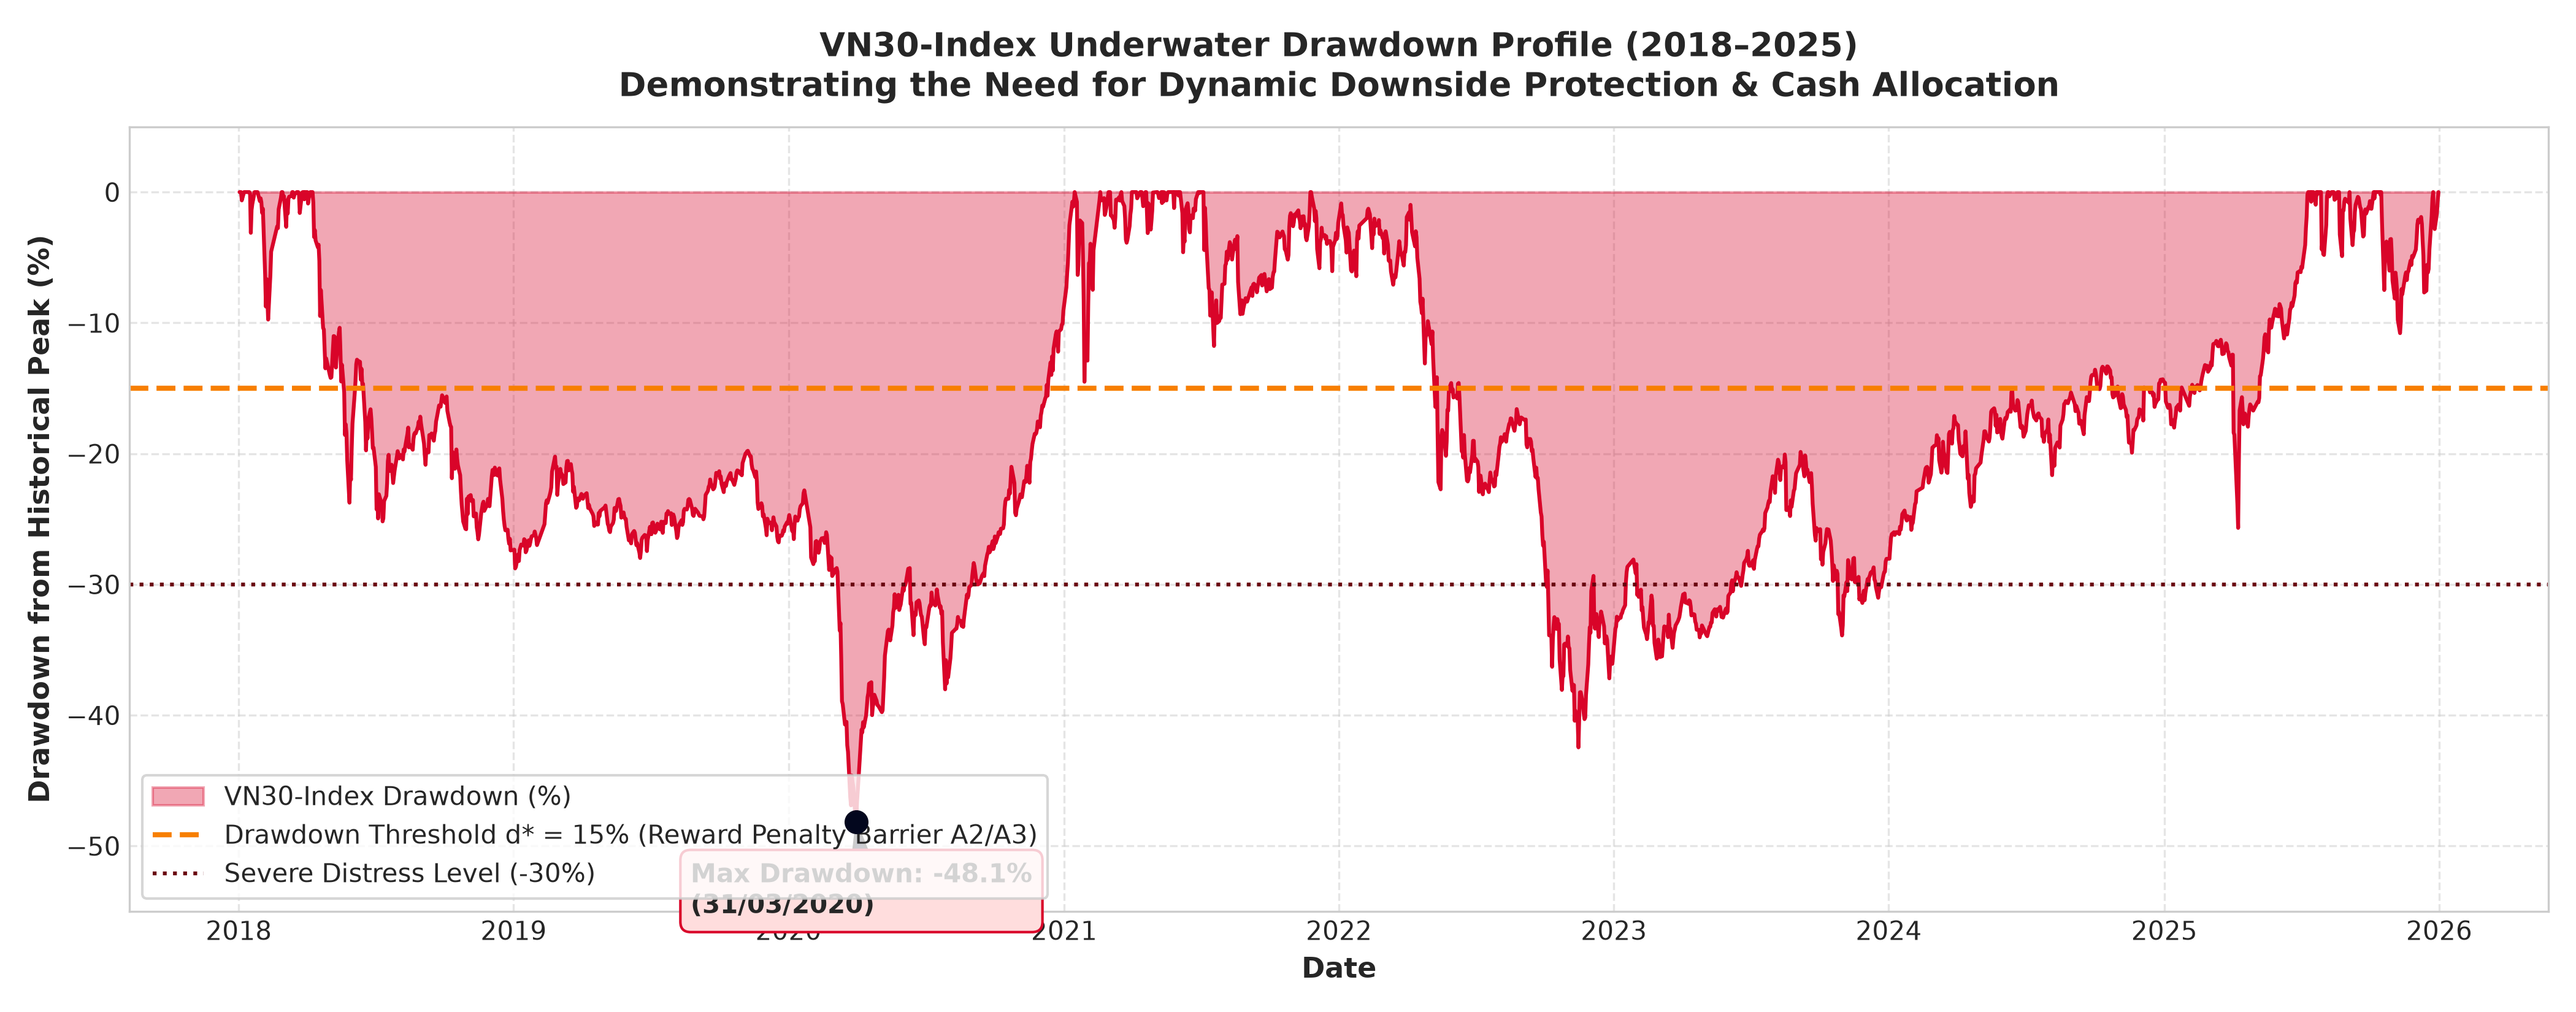
\includegraphics[width=\textwidth]{figures/06_vn30_underwater_drawdown.png}\\
      \vspace{0.5ex}
      {\scriptsize \textbf{Biểu đồ sụt vốn rổ VN30 (2018--2025):} Các hố sâu thể hiện tài sản sụt giảm 30\%--50\% nếu không biết thoát sang tiền mặt.}
    \end{column}
  \end{columns}
\end{frame}

% ------------------------------------------------------------------------------
% Slide 5: HOSE Market Rules (Simple, relatable)
% ------------------------------------------------------------------------------
\begin{frame}{3. Sàn Chứng Khoán Việt Nam (HOSE) Có Gì Đặc Thù?}
  Nếu mang nguyên mẫu bot AI của Mỹ về Việt Nam chạy, bot sẽ \textbf{"cháy tài khoản"} vì 5 luật chơi đặc thù của sàn HOSE:

  \vspace{1ex}
  \begin{table}[h]
    \centering
    \small
    \begin{tabular}{p{2.6cm} p{1.6cm} p{8.8cm}}
      \toprule
      \textbf{Luật Sàn HOSE} & \textbf{Quy định} & \textbf{Ý nghĩa đời thường (Tại sao bot dễ chết?)} \\
      \midrule
      \textbf{Chu kỳ thanh toán} & \textbf{T+2} & Mua hôm nay thì \textbf{2 ngày sau} cổ phiếu mới về để bán. Nếu vừa mua xong cổ phiếu giảm sàn, bot phải trơ mắt đứng nhìn, không được cắt lỗ ngay! \\
      \midrule
      \textbf{Biên độ giá} & \textbf{$\pm 7\%$} & Mỗi ngày tối đa chỉ tăng hoặc giảm 7\%. Khi giảm kịch sàn ($-7\%$), trắng bên mua, muốn bán tháo cũng không ai mua. \\
      \midrule
      \textbf{Đơn vị mua} & \textbf{Lô 100} & Bắt buộc mua chẵn từng 100 cổ phiếu, không được mua lẻ 15, 30 cổ phiếu. \\
      \midrule
      \textbf{Thuế \& Phí} & \textbf{~0.40\%} & Bán mất 0.1\% thuế + phí mua bán 0.15\%. Nếu bot đảo danh mục liên tục mỗi ngày, phí giao dịch sẽ "bào mòn" hết vốn. \\
      \midrule
      \textbf{Không bán khống} & \textbf{Long-Only} & Không được mượn hàng bán trước. Khi thị trường sập, cách phòng thủ duy nhất là \textbf{ôm Tiền mặt}. \\
      \bottomrule
    \end{tabular}
  \end{table}
\end{frame}

% ------------------------------------------------------------------------------
% Slide 6: Our Proposal (Bot that understands risk)
% ------------------------------------------------------------------------------
\begin{frame}{4. Ý Tưởng Đề Tài: Xây Dựng Bot AI "Biết Sợ Rủi Ro"}
  Thay vì dạy AI chỉ biết ham kiếm lời, đề tài xây dựng tác tử học theo triết lý:
  \begin{center}
    {\Large \color{MainNavy}\textbf{"Bảo toàn vốn trước, tối ưu hóa lợi nhuận sau!"}}
  \end{center}

  \vspace{1ex}
  \begin{columns}[t]
    \begin{column}{0.32\textwidth}
      \begin{block}{\textbf{1. Phạt Sụt Vốn Nặng}}
        \small
        Mỗi khi tài khoản bị sụt giảm quá $15\%$, hệ thống áp dụng \textbf{mức phạt cực nặng} vào điểm số của AI để ép nó phải tránh xa các mã rủi ro.
      \end{block}
    \end{column}

    \begin{column}{0.32\textwidth}
      \begin{block}{\textbf{2. Tâm Lý "Sợ Lỗ"}}
        \small
        Áp dụng lý thuyết kinh tế học hành vi (\textit{Prospect Theory}): Nỗi đau khi mất 10 triệu lớn gấp đôi niềm vui khi kiếm được 10 triệu $\to$ Bot ưu tiên phòng vệ.
      \end{block}
    \end{column}

    \begin{column}{0.32\textwidth}
      \begin{block}{\textbf{3. Hầm Trú Ẩn Tiền Mặt}}
        \small
        Cho phép Bot tự do giữ tiền mặt. Khi nhận thấy thị trường xấu, Bot chủ động \textbf{chuyển vốn về 100\% Tiền mặt} để đứng ngoài quan sát bão.
      \end{block}
    \end{column}
  \end{columns}
\end{frame}

% ------------------------------------------------------------------------------
% ------------------------------------------------------------------------------
% Slide 7: Portfolio Allocation Analogy (100% Pie)
% ------------------------------------------------------------------------------
\begin{frame}{5. Bot Ra Quyết Định Như Thế Nào? (Nguyên Lý "Chiếc Bánh 100\%")}
  \begin{columns}[t]
    \begin{column}{0.50\textwidth}
      \begin{block}{Chiếc bánh danh mục 100\%}
        \small
        \begin{itemize}
          \item Gồm: \textbf{30 cổ phiếu VN30 + Tiền mặt}.
          \item Mỗi ngày, Bot quan sát thị trường và chia lại tỷ trọng:
        \end{itemize}
        \vspace{0.5ex}
        \centering
        \textbf{\color{AccentCyan}Tỷ trọng cổ phiếu $+$ Tiền mặt $= 100\%$}
      \end{block}

      \vspace{-0.5ex}
      \successcard{Hành động thông minh}{
        \small
        \begin{itemize}
          \item \textbf{Khi thị trường tăng:} Chia nhiều cho mã khỏe (VD: 30\% FPT, 20\% HPG, 10\% Tiền mặt).
          \item \textbf{Khi thị trường bão:} Rút về tiền mặt an toàn (VD: 80\% Tiền mặt, 20\% mã phòng thủ).
        \end{itemize}
      }
    \end{column}

    \begin{column}{0.48\textwidth}
      \begin{block}{Bộ "Giác Quan" Của Bot (Nó nhìn thấy gì?)}
        \small
        Mỗi ngày, Bot quan sát các thông tin chuẩn hóa:
        \begin{itemize}
          \item Giá đóng cửa và khối lượng khớp lệnh.
          \item Sức mạnh xu hướng giá (\textbf{RSI}).
          \item Tín hiệu đảo chiều xu hướng (\textbf{MACD}).
          \item Độ biến động rủi ro (\textbf{ATR, Bollinger Bands}).
          \item Trạng thái danh mục hiện tại đang cầm gì.
        \end{itemize}
      \end{block}
    \end{column}
  \end{columns}
\end{frame}

% ------------------------------------------------------------------------------
% Slide 8: Architecture Diagram
% ------------------------------------------------------------------------------
\begin{frame}{6. Kiến Trúc Hoạt Động 4 Tầng Của Hệ Thống}
  \begin{center}
    \begin{tikzpicture}[
      node distance=0.8cm and 0.9cm,
      box/.style={rectangle, draw=SecondaryNavy, fill=BgSoftGray, text=DarkText, rounded corners=3pt, minimum width=2.6cm, minimum height=1.3cm, align=center, font=\footnotesize, line width=1pt},
      activebox/.style={rectangle, draw=MainNavy, fill=SecondaryNavy!15, text=MainNavy, rounded corners=3pt, minimum width=2.6cm, minimum height=1.3cm, align=center, font=\footnotesize\bfseries, line width=1.2pt},
      arrow/.style={-{Stealth[scale=1.1]}, line width=1.5pt, color=AccentCyan}
    ]
      \node[box] (data) {\textbf{Tầng 1: Dữ Liệu}\\Thu thập 30 mã VN30\\(vnstock \& yfinance)};
      \node[box, right=of data] (feat) {\textbf{Tầng 2: Xử Lý}\\Làm sạch, khử nhiễu\\Tính 11 chỉ báo kỹ thuật};
      \node[activebox, right=of feat] (env) {\textbf{Tầng 3: Sàn Giả Lập}\\Gymnasium Env\\Khóa T+2, biên độ $\pm 7\%$};
      \node[box, right=of env] (agent) {\textbf{Tầng 4: Bộ Não AI}\\Thuật toán PPO \& SAC\\Tối ưu tỷ trọng an toàn};

      \draw[arrow] (data) -- (feat);
      \draw[arrow] (feat) -- (env);
      \draw[arrow] (env) -- (agent);
      \draw[arrow, dashed, color=AlertCrimson] (agent.south) -- ++(0,-0.4) -| node[pos=0.25, below, font=\scriptsize] {Hành động phân bổ tỷ trọng mới} (env.south);
    \end{tikzpicture}
  \end{center}

  \vspace{0.5ex}
  \begin{columns}[t]
    \begin{column}{0.48\textwidth}
      \begin{block}{\textbf{Điểm mạnh của kiến trúc}}
        \footnotesize
        \begin{itemize}
          \item \textbf{Tách biệt độc lập:} Tầng dữ liệu, sàn giả lập và bộ não AI hoạt động module hóa, dễ bảo trì và nâng cấp.
          \item \textbf{Khử rò rỉ tương lai:} Đảm bảo bot chỉ nhìn dữ liệu quá khứ đến ngày $t$, tuyệt đối không "nhìn trộm" tương lai ngày $t+1$.
        \end{itemize}
      \end{block}
    \end{column}

    \begin{column}{0.48\textwidth}
      \begin{block}{\textbf{Kiểm định tự động (CI/CD)}}
        \footnotesize
        \begin{itemize}
          \item Toàn bộ mã nguồn được bao bọc bởi hệ thống kiểm thử tự động (\texttt{pytest}).
          \item Tự động xác thực tính toán đặc trưng và độ chuẩn xác của dữ liệu trước khi nạp vào AI.
        \end{itemize}
      \end{block}
    \end{column}
  \end{columns}
\end{frame}

% ------------------------------------------------------------------------------
% Slide 9: Gymnasium Environment explained simply
% ------------------------------------------------------------------------------
\begin{frame}{7. Sàn Đấu Giả Lập: Môi Trường Gymnasium}
  \begin{columns}[t]
    \begin{column}{0.50\textwidth}
      \begin{block}{Gymnasium là gì?}
        \small
        \begin{itemize}
          \item Là thư viện chuẩn thế giới của OpenAI / Farama để dựng \textbf{"sân chơi giả lập"} cho AI.
          \item Giống như buồng lái giả lập phi công: Bot được vào tập lái hàng triệu lần, tự mắc sai lầm, tự sụt tài khoản mà **không mất đồng tiền thật nào**.
        \end{itemize}
      \end{block}

      \vspace{-0.5ex}
      \begin{block}{Vòng lặp mỗi ngày của sàn giả lập}
        \small
        \begin{enumerate}
          \item Sàn gửi cho Bot ảnh chụp bảng điện tử hôm nay.
          \item Bot gửi lại tỷ trọng phân bổ mới.
          \item Sàn trừ thuế 0.1\%, trừ phí 0.15\%, khóa cổ phiếu $T+2$.
          \item Sàn chấm điểm thưởng phạt cho Bot.
        \end{enumerate}
      \end{block}
    \end{column}

    \begin{column}{0.48\textwidth}
      \alertcard{Tại sao sàn giả lập này khác biệt?}{
        \small
        \begin{itemize}
          \item Hầu hết các thư viện AI trên mạng (như FinRL) chỉ mô phỏng thị trường Mỹ: mua bán được ngay, bán khống thoải mái.
          \item \textbf{Đề tài tự xây dựng môi trường thuần Việt:} Khóa chặt quy tắc thanh toán $T+2$ và chặn trần sàn $\pm 7\%$ của sàn HOSE.
          \item Đạt chuẩn kiểm định \texttt{check\_env} nghiêm ngặt của Gymnasium quốc tế.
        \end{itemize}
      }
    \end{column}
  \end{columns}
\end{frame}

% ------------------------------------------------------------------------------
% Slide 10: Two AI Algorithms (PPO & SAC)
% ------------------------------------------------------------------------------
\begin{frame}{8. Hai "Học Trò AI": Thuật Toán PPO và SAC}
  Đề tài thử nghiệm và so tài giữa hai thuật toán Học tăng cường hàng đầu hiện nay:

  \vspace{1ex}
  \begin{columns}[t]
    \begin{column}{0.48\textwidth}
      \begin{block}{\textbf{PPO (Proximal Policy Optimization)}}
        \centering
        {\large \color{AccentCyan}\textbf{"Học Trò Cẩn Trọng \& Điềm Tĩnh"}}
        \vspace{0.8ex}
        \begin{itemize}
          \item \textbf{Cách học:} Mỗi lần rút kinh nghiệm, PPO chỉ điều chỉnh chiến thuật một bước rất nhỏ, không bao giờ thay đổi đột ngột.
          \item \textbf{Ưu điểm:} Rất ổn định, không bị "loạn chưởng" khi thị trường rung lắc mạnh.
          \item \textbf{Phù hợp:} Nhà đầu tư thích sự an toàn, bảo vệ vốn đều đặn.
        \end{itemize}
      \end{block}
    \end{column}

    \begin{column}{0.48\textwidth}
      \begin{block}{\textbf{SAC (Soft Actor-Critic)}}
        \centering
        {\large \color{SuccessGreen}\textbf{"Học Trò Linh Hoạt \& Khám Phá"}}
        \vspace{0.8ex}
        \begin{itemize}
          \item \textbf{Cách học:} Vừa tìm cách tối ưu danh mục, vừa tối đa hóa "sự tò mò" (Entropy) để liên tục thử nghiệm cơ hội mới.
          \item \textbf{Ưu điểm:} Thích ứng siêu nhanh khi thị trường bất ngờ đảo chiều xu hướng.
          \item \textbf{Phù hợp:} Nắm bắt nhanh các chu kỳ xoay vòng dòng tiền giữa các nhóm ngành.
        \end{itemize}
      \end{block}
    \end{column}
  \end{columns}
\end{frame}

% ------------------------------------------------------------------------------
% Slide 9: Evaluation & KPI Targets
% ------------------------------------------------------------------------------
\begin{frame}{9. Làm Sao Biết Bot Đầu Tư Hiệu Quả? (Bảng Chỉ Tiêu KPI)}
  Đề tài không chỉ nhìn vào số tiền lãi, mà chấm điểm dựa trên \textbf{chất lượng quản trị rủi ro}:

  \vspace{1ex}
  \begin{table}[h]
    \centering
    \small
    \begin{tabular}{p{3.2cm} c p{7.5cm}}
      \toprule
      \textbf{Chỉ Số Đánh Giá} & \textbf{Mục Tiêu Bot} & \textbf{Ý Nghĩa Dễ Hiểu} \\
      \midrule
      \textbf{Mức sụt vốn tối đa} (Max Drawdown) & $\mathbf{\le 15\%}$ & Lúc thị trường sập $40\%-50\%$, danh mục của Bot cam kết sụt giảm không quá $15\%$. \\
      \midrule
      \textbf{Chỉ số Sharpe} & $\mathbf{\ge 1.2}$ & Đo lường mức sinh lời trên mỗi đơn vị rủi ro (Chỉ số của VN-Index thường $< 0.5$). \\
      \midrule
      \textbf{Chỉ số Sortino} & $\mathbf{\ge 1.8}$ & Tương tự Sharpe nhưng chỉ phạt khi tài sản bị lỗ (không phạt những đợt tăng giá mạnh). \\
      \midrule
      \textbf{Chi phí đảo vị thế} (Turnover Cost) & $\mathbf{< 2\%}$/năm & Bot không được mua bán điên cuồng mỗi ngày làm thất thoát tiền cho phí môi giới. \\
      \bottomrule
    \end{tabular}
  \end{table}

  \vspace{0.5ex}
  \begin{center}
    {\footnotesize \textbf{Phương pháp kiểm tra:}} Kiểm định độc lập trên dữ liệu chưa từng thấy (\textit{Out-of-Sample}) từ năm 2022 đến 2025.
  \end{center}
\end{frame}

% ------------------------------------------------------------------------------
% Slide 10: EDA & Diversification
% ------------------------------------------------------------------------------
\begin{frame}{10. Phân Tích Thực Nghiệm: "Không Bỏ Trứng Vào Một Giỏ"}
  \begin{columns}[c]
    \begin{column}{0.48\textwidth}
      \centering
      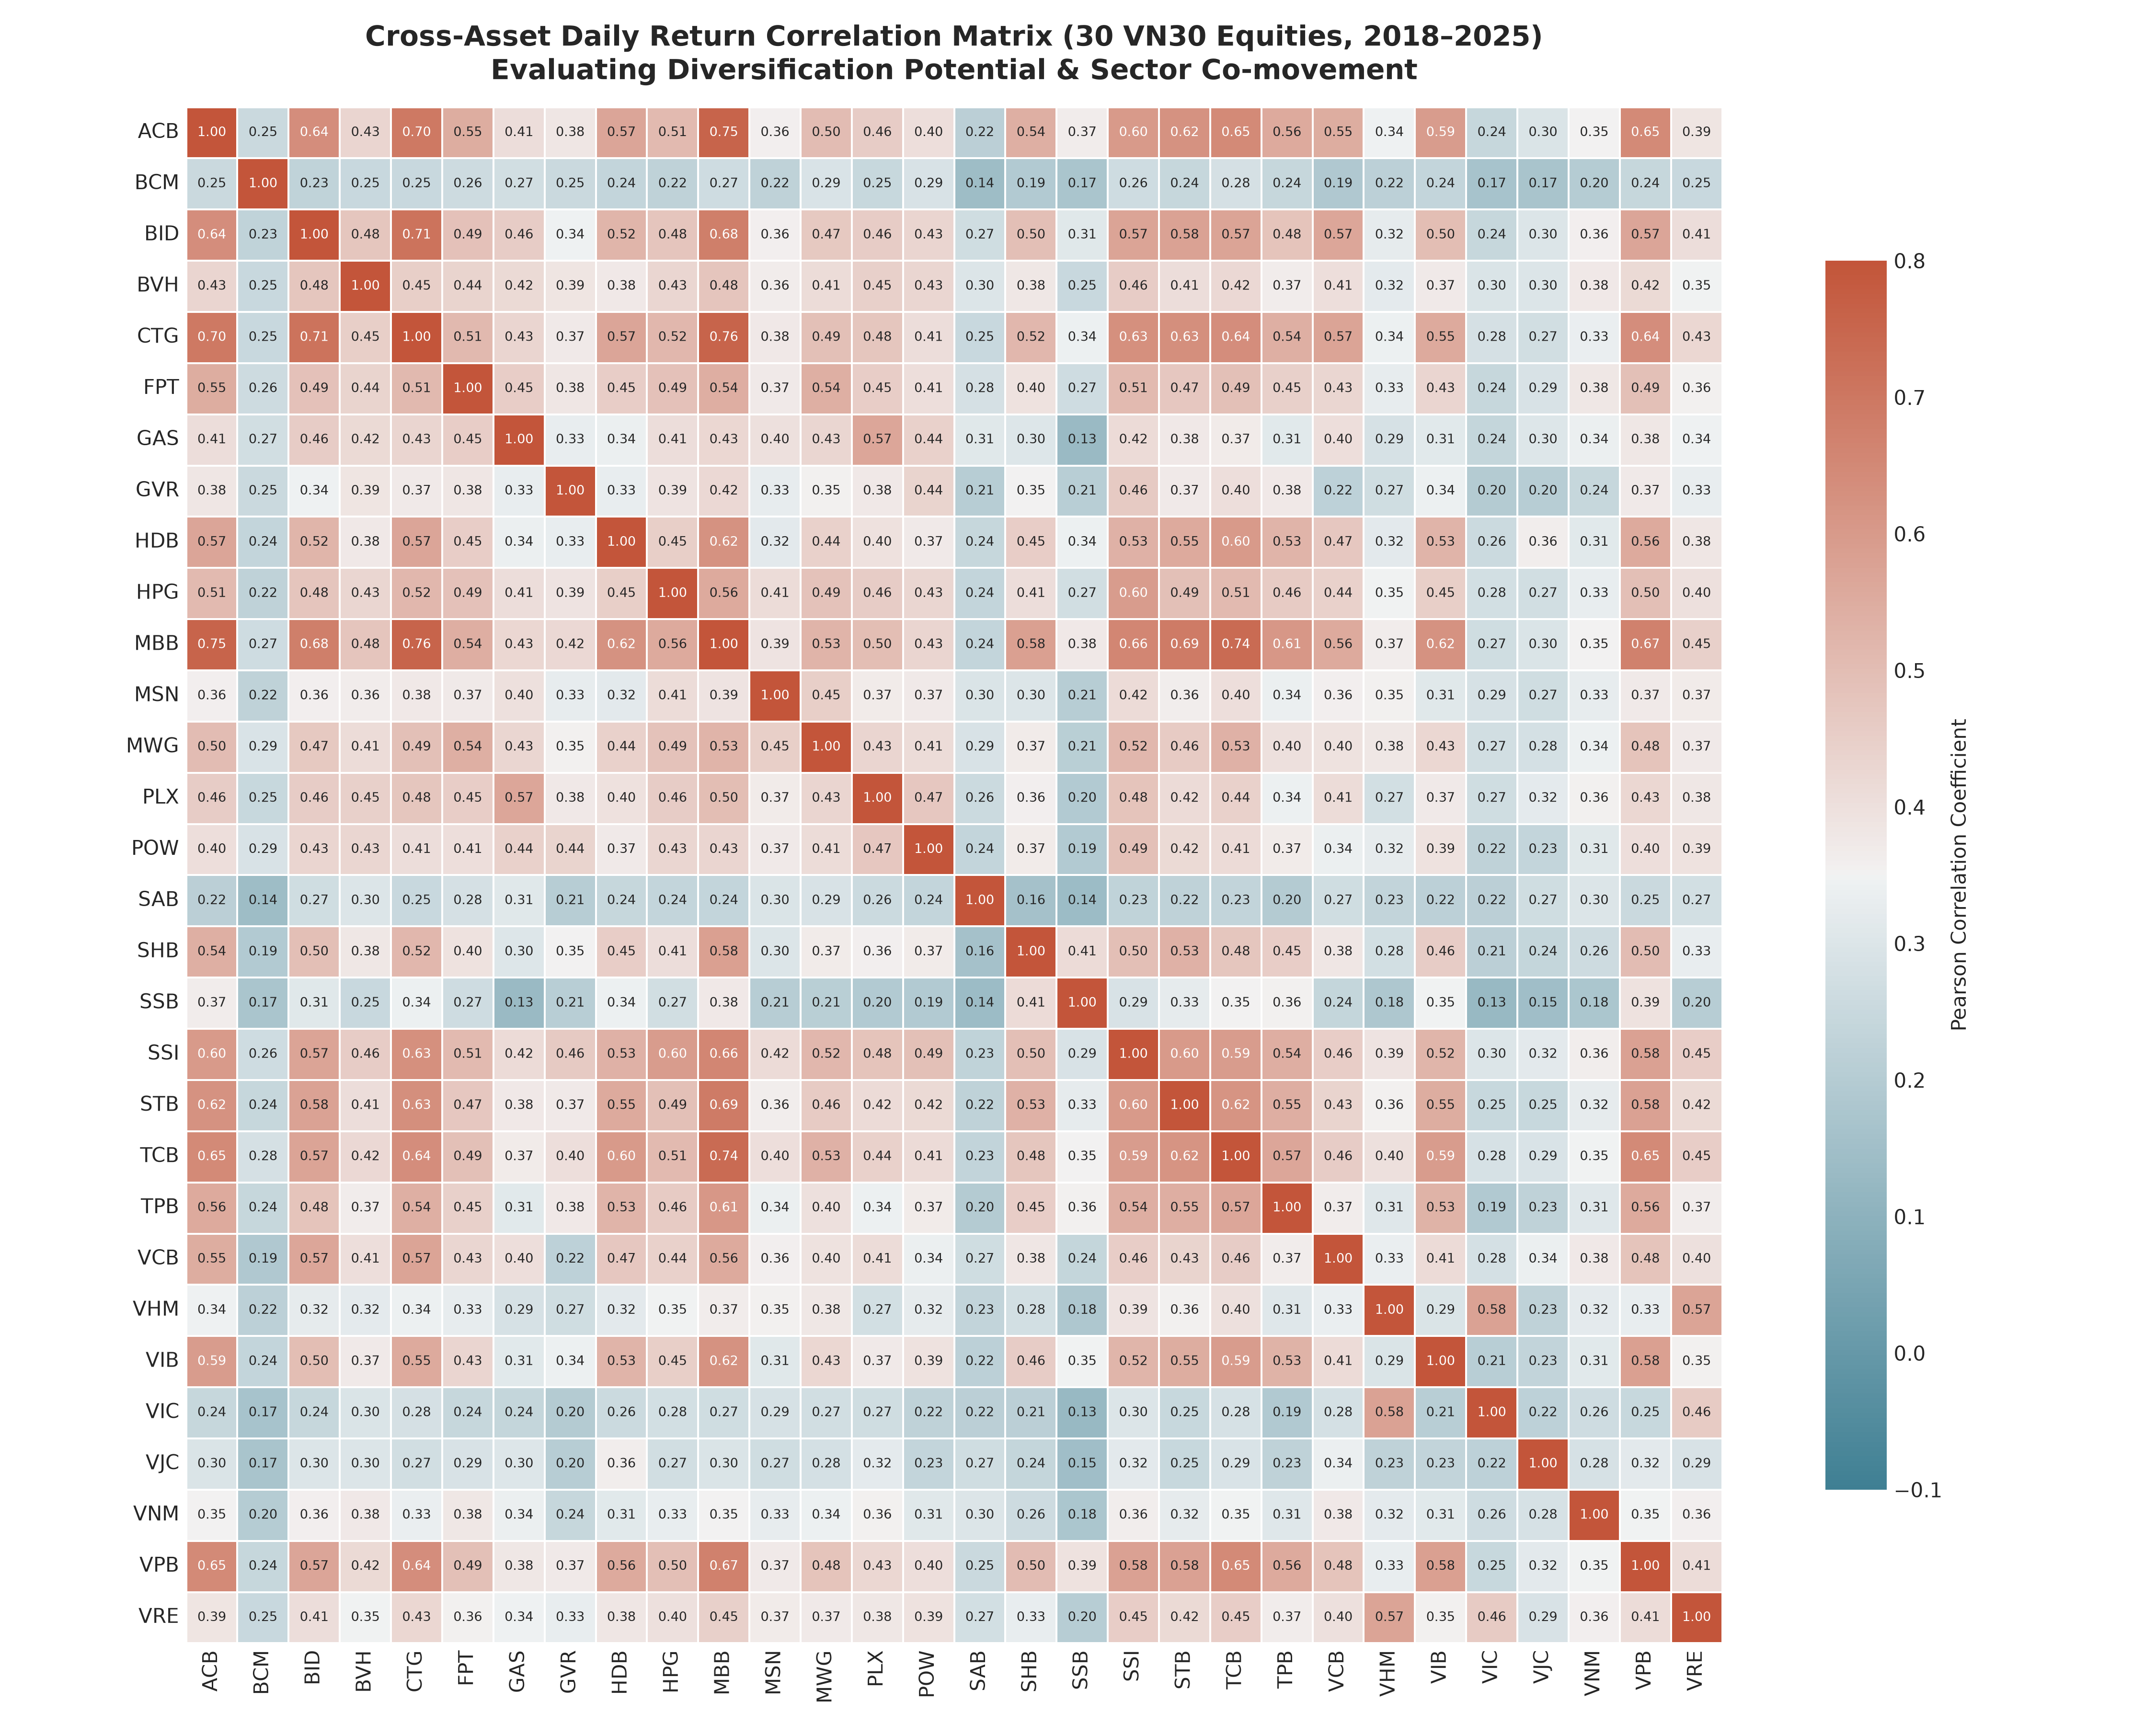
\includegraphics[width=\textwidth]{figures/02_vn30_correlation_matrix.png}\\
      \vspace{0.5ex}
      {\scriptsize \textbf{Ma trận tương quan rổ VN30:} Các ô màu nhạt thể hiện các cặp cổ phiếu ít phụ thuộc lẫn nhau $\to$ Rất tốt để phân tán rủi ro.}
    \end{column}

    \begin{column}{0.50\textwidth}
      \begin{block}{Tại sao lại là rổ VN30?}
        \begin{itemize}
          \item Tập trung 30 doanh nghiệp đầu ngành tại Việt Nam (HPG, FPT, VNM, VHM, VCB...).
          \item Thanh khoản dồi dào, chiếm hơn 80\% vốn hóa toàn thị trường chứng khoán.
          \item Tránh được rủi ro bị "thao túng giá" (lái giá) như các cổ phiếu Penny nhỏ lẻ.
        \end{itemize}
      \end{block}

      \successcard{Nguyên lý phân tán rủi ro}{
        \small
        Nếu chỉ mua một ngành (ví dụ Bất động sản), khi ngành đó gặp khó thì tài khoản sẽ sập theo. Bot sẽ phân bổ tiền sang Ngân hàng, Công nghệ, Bán lẻ và Tiền mặt để cân bằng rủi ro.
      }
    \end{column}
  \end{columns}
\end{frame}

% ------------------------------------------------------------------------------
% Slide 11: Current Progress
% ------------------------------------------------------------------------------
\begin{frame}{11. Tiến Độ Hiện Tại}
  \begin{columns}[t]
    \begin{column}{0.48\textwidth}
      \begin{block}{\textbf{1. Chuẩn Bị Dữ Liệu}}
        \small
        \begin{itemize}
          \item Đã cào và làm sạch dữ liệu lịch sử của \textbf{30 mã cổ phiếu VN30} (giai đoạn 2018--2025).
          \item Xử lý ngày nghỉ lễ, ngày đặc biệt và các mốc cổ phiếu mới chuyển sàn vào rổ.
        \end{itemize}
      \end{block}
    \end{column}

    \begin{column}{0.48\textwidth}
      \begin{block}{\textbf{2. Chỉ Báo \& Khung Giả Lập}}
        \small
        \begin{itemize}
          \item Đã tính sẵn các chỉ số kỹ thuật cơ bản: RSI, MACD, Bollinger Bands, mức biến động giá.
          \item Đã dựng khung môi trường giả lập Gymnasium ban đầu để chuẩn bị nạp dữ liệu cho mô hình.
        \end{itemize}
      \end{block}
    \end{column}
  \end{columns}

  \vspace{1.5ex}
  \begin{center}
    \footnotesize \color{SecondaryNavy}\textbf{Đánh giá:} Đã hoàn tất khâu chuẩn bị dữ liệu đầu vào, sẵn sàng bước vào phát triển môi trường và huấn luyện mô hình.
  \end{center}
\end{frame}

% ------------------------------------------------------------------------------
% Slide 12: Next Phase
% ------------------------------------------------------------------------------
\begin{frame}{12. Giai Đoạn Tiếp Theo}
  Trong giai đoạn tới, nhóm tập trung thực hiện \textbf{02 nhiệm vụ trọng tâm}:

  \vspace{1.5ex}
  \begin{columns}[t]
    \begin{column}{0.48\textwidth}
      \begin{block}{\textbf{Nhiệm Vụ 1: Hoàn Thiện Môi Trường}}
        \small
        \begin{itemize}
          \item Khóa chặt các quy tắc thực tế của sàn HOSE: hàng đợi thanh toán $T+2$, biên độ trần/sàn $\pm 7\%$.
          \item Tích hợp cơ chế phạt khi sụt giảm vốn để ép Bot học cách ưu tiên bảo vệ tài sản.
        \end{itemize}
      \end{block}
    \end{column}

    \begin{column}{0.48\textwidth}
      \begin{block}{\textbf{Nhiệm Vụ 2: Huấn Luyện Thử Nghiệm}}
        \small
        \begin{itemize}
          \item Chạy thử nghiệm 2 thuật toán \textbf{PPO và SAC} trên dữ liệu lịch sử.
          \item Đánh giá hành vi của Bot: Xem Bot có biết tự động tăng tỷ trọng Tiền mặt khi thị trường đi xuống hay không.
        \end{itemize}
      \end{block}
    \end{column}
  \end{columns}

  \vspace{1.5ex}
  \begin{center}
    \footnotesize \color{SecondaryNavy}\textbf{Mục tiêu:} Có được mô hình cơ sở đầu tiên biết tự co cụm phòng thủ trước khủng hoảng.
  \end{center}
\end{frame}

\end{document}

